% LuaLaTeX / Windows. Rebuilt in response to Print (8).pdf.
% LuaLaTeX, Windows. Revised against the handwritten review on 2026-09-22.
\documentclass[a4paper,11pt]{ltjsarticle}
\usepackage[top=19mm,bottom=19mm,left=20mm,right=20mm,headheight=16pt,headsep=6mm]{geometry}
\usepackage{luatexja-fontspec}
\setmainfont[Path=C:/Windows/Fonts/,BoldFont=timesbd.ttf,ItalicFont=timesi.ttf,BoldItalicFont=timesbi.ttf]{times.ttf}
\setsansfont[Path=C:/Windows/Fonts/,BoldFont=arialbd.ttf]{arial.ttf}
\setmainjfont[Path=C:/Windows/Fonts/,BoldFont=yumindb.ttf]{yumin.ttf}
\setsansjfont[Path=C:/Windows/Fonts/,BoldFont=YuGothB.ttc]{YuGothM.ttc}
\usepackage{amsmath,amssymb,graphicx,booktabs,tabularx,array}
\usepackage{xcolor,tikz,tcolorbox,fancyhdr,enumitem}
\usetikzlibrary{arrows.meta,positioning,calc}
\definecolor{navy}{HTML}{203C55}\definecolor{teal}{HTML}{138B86}
\definecolor{orange}{HTML}{D77932}\definecolor{pale}{HTML}{F0F6F7}
\definecolor{muted}{HTML}{657987}\definecolor{light}{HTML}{D6E1E5}
\usepackage[unicode,colorlinks=true,linkcolor=teal,urlcolor=teal,citecolor=teal]{hyperref}
\hypersetup{pdftitle={G22・G55・G70の構造からCIMの解をどう理解するか・第2回改訂版},pdfauthor={研究調査資料}}
\graphicspath{{figures/}}
\pagestyle{fancy}\fancyhf{}
\fancyhead[L]{\small\sffamily\color{muted}グラフ構造・Max-Cut・CIM}
\fancyhead[R]{\small\sffamily\color{muted}第2回改訂版 / 2026.09.22}
\fancyfoot[L]{\footnotesize\color{muted}構造の理解と先行研究の精読}
\fancyfoot[R]{\sffamily\color{navy}\thepage}
\renewcommand{\headrulewidth}{0.3pt}
\setlength{\parindent}{1em}\setlength{\parskip}{3pt}
\renewcommand{\baselinestretch}{1.06}
\renewenvironment{center}{\par\vspace{2pt}\centering}{\par\vspace{2pt}}
\setlist[itemize]{leftmargin=1.5em,itemsep=3pt,topsep=4pt}
\setlist[enumerate]{leftmargin=1.8em,itemsep=4pt,topsep=4pt}
\newcommand{\pagehead}[3]{\pdfbookmark[0]{#2}{p\thepage}\noindent{\sffamily\small\color{teal}#1}\par\vspace{1mm}\noindent{\sffamily\bfseries\LARGE\color{navy}#2}\par\vspace{1mm}\noindent{\color{muted}#3}\par\vspace{2mm}}
\newcommand{\sub}[1]{\par\vspace{2mm}\noindent{\sffamily\bfseries\large\color{navy}#1}\par}
\newcommand{\figcap}[2]{\par\vspace{1mm}\noindent{\small\sffamily\color{teal}図#1}\quad{\small #2}\par\vspace{2mm}}
\newcommand{\source}[1]{\par\noindent{\footnotesize\color{muted}出典・根拠：#1}\par}
\newcommand{\pic}[2]{\begin{center}\includegraphics[width=\textwidth,height=#2,keepaspectratio]{#1}\end{center}}
\newtcolorbox{point}[1]{colback=pale,colframe=teal,boxrule=.5pt,arc=1.5mm,left=3mm,right=3mm,top=2mm,bottom=2mm,title=#1,coltitle=white,fonttitle=\sffamily\bfseries}
\newtcolorbox{caution}[1]{colback=orange!5,colframe=orange!70,boxrule=.4pt,arc=1.5mm,left=3mm,right=3mm,top=2mm,bottom=2mm,title=#1,coltitle=navy,colbacktitle=orange!16,fonttitle=\sffamily\bfseries}
\tikzset{box/.style={draw=light,fill=pale,rounded corners=2mm,align=center,font=\sffamily\small,text=navy,minimum height=14mm,text width=33mm,inner sep=3mm},flow/.style={-{Stealth[length=2.5mm]},thick,draw=teal},dot/.style={circle,fill=teal,inner sep=0pt,minimum size=3mm}}

\newcommand{\nextstep}[1]{\vfill\begin{point}{ここまでの答えと、次の問い}#1\end{point}}
\begin{document}
\thispagestyle{empty}\pdfbookmark[0]{目的と読み方}{cover}
\noindent{\sffamily\bfseries\color{teal}\large RESEARCH NOTE / 第2回改訂}\hfill{\sffamily\color{muted}2026年9月22日}\par
\vspace{10mm}
\noindent{\sffamily\bfseries\fontsize{27}{37}\selectfont\color{navy}G22・G55・G70の構造から\\CIMの解をどう理解するか}\par
\vspace{6mm}
\noindent{\Large 何を調べたいのか → なぜその指標か → 何が分かるか}\par
\vspace{4mm}\noindent\textcolor{teal}{\rule{\textwidth}{1.1pt}}

\sub{出発点は「CIMが作る解の違いを説明したい」}
CIMが同じように動いても、入力がG22・G55・G70のどれかによって、得られる解の傾向は変わる。その違いを考えるため、まず\textbf{グラフのどの部分を分けて考えられ、どこを詳しく調べる必要があるか}を整理する。

将来はGAやSAへ渡す候補の評価に使いたい。しかし、グラフだけから計算する値は、同じグラフ上の全候補で共通である。今回は、候補を採点する前の土台として、\textbf{構造とCIM出力を対応させて読む方法}に集中する。

\begin{center}
\begin{tikzpicture}
\node[box,text width=39mm] (a) at (0,0) {\textbf{① 分けて考える}\\木や橋でつながる部分\\3--7ページ};
\node[box,text width=39mm] (b) at (5.3,0) {\textbf{② 残る問題を読む}\\次数・閉路・固有値\\8--11ページ};
\node[box,text width=39mm] (c) at (10.6,0) {\textbf{③ 研究へつなぐ}\\先行研究から観測を選ぶ\\12--15ページ};
\draw[flow](a)--(b);\draw[flow](b)--(c);
\end{tikzpicture}
\end{center}
\figcap{1}{この資料の道順。用語を順に覚えるためではなく、「CIMの出力のどこを見るか」を決めるために読む。2ページで共通の得点を確認する。}

\sub{なぜ「橋」や「core」を説明するのか}
木や橋の部分では、他の部分の得点を落とさずに、すべての辺をcutできる。そのため、CIMの未cut辺を\textbf{木・橋の側}と\textbf{残った中心部分}に分けると、改善の余地がどこにあるかを区別できる。橋やcoreは、その分け方を説明するために登場する。

\begin{caution}{最初に区別しておくこと}
「構造上、分けて解ける」ことと、「現在のCIMやGAが容易に良い解を出す」ことは別である。前者は数学と構造の話、後者は実際の探索結果の話として扱う。
\end{caution}
\vfill
\noindent{\small\color{muted}対象入力：本リポジトリのG22・G55・G70。手書き修正「Print (8).pdf」を反映。\\今回は資料の再構成と構造の追加集計。CIM・GA・SAの新たな性能実験は行っていない。}

\newpage
\pagehead{01 / 共通の得点を確認する}{異なる組を結ぶ辺が、Max-Cutの得点}{この得点を、後で「部分ごと」に分けて考える。}
ここでいう\textbf{三つの入力はG22・G55・G70}である。ローカルの入力ファイルでは、いずれも全辺の重みが$+1$だった。したがって今回は、異なる組を結ぶ辺1本を1点と数える。
\pic{cut_example.pdf}{49mm}
\figcap{2}{同じ説明用グラフの二つの割当て。緑と紺は二つの組、オレンジはcut辺、灰色は未cut辺。左は2点、右は4点。}

\sub{式の記号を、一つずつ読む}
\noindent\begin{tabularx}{\textwidth}{@{}lX@{}}\toprule
$V$ & 頂点の集合。各頂点に$+1$か$-1$を割り当てる。\\
$E$ & 実際に存在する辺の集合。$\{i,j\}\in E$は「頂点$i,j$を結ぶ辺がある」の意味。全頂点対の集合ではない。\\
$s_i$ & 頂点$i$の組を表す符号。$+1$と$-1$が二つの組に対応する。\\
$w_{ij}$ & 辺$\{i,j\}$の重み。今回の三つの入力では1。\\\bottomrule
\end{tabularx}
\[
C_G(s)=\sum_{\{i,j\}\in E}w_{ij}\frac{1-s_is_j}{2}
\]
\begin{center}
\begin{tabular}{lccc}\toprule
両端の組 & $s_is_j$ & $(1-s_is_j)/2$ & 今回の得点\\\midrule
同じ組 & $+1$ & $0$ & 0点\\
異なる組 & $-1$ & $1$ & 1点\\\bottomrule
\end{tabular}
\end{center}
\textbf{符号の積}と\textbf{得点}は別である。異なる組で$-1$になるのは積$s_is_j$で、得点は式に代入して$1$となる。各辺は一度だけ足す。

\begin{point}{全反転で「変わらない」のは、どの辺か}
全頂点を反転すれば、全辺の得点が変わらない。\textbf{一部分だけ}を全反転した場合、その\textbf{内部の辺}の得点は変わらないが、\textbf{外へ出る辺}の得点は変わり得る。この違いが、橋の説明の鍵になる。
\end{point}
\source{入力の重みと構造は[7]。図と符号の説明は本資料で作成。}

\newpage
\pagehead{02 / 分けられる場所を探す}{橋と関節点は、問題の「切れ目」を示す}{ここでの目的は、別々に解いてから組み合わせられる場所を探すこと。}
大きなグラフを小さな問題へ分けられれば、どの部分で得点を失ったかを個別に調べられる。最初に、\textbf{1本の辺}または\textbf{1個の頂点}を境に分かれる形を見る。
\pic{bridge_articulation.pdf}{83mm}
\figcap{3}{説明用のグラフ。緑は頂点、灰色は辺、オレンジは除去する対象。上段は辺の除去、下段は頂点と接続辺の除去。ここで点の色は解の割当てではない。}

\sub{橋：その辺が唯一の通り道}
上段の中央の辺を除くと、左と右を行き来できなくなる。このような辺が\textbf{橋}である。三角形の辺を1本除いても、他の2本を通って戻れるため、それらは橋ではない。

\sub{関節点：その頂点が唯一の通り道}
下段では、中央の頂点とそこにつながる辺を除くと左右が分かれる。このような頂点が\textbf{関節点}である。中央につながる各辺には三角形内の迂回路があるため、この例に橋はない。

\begin{point}{何に使えるか}
Max-Cutでは、橋の左右をそれぞれ良く解いた後、片側の符号を全反転してつなげられる。関節点で分けた場合も、共有点の符号を合わせれば、各部分の最適な得点を保って結合できる。[2]
\end{point}
\noindent\textcolor{teal}{次は、最も単純な「橋が1本」の場合を数値で確かめる。}

\newpage
\pagehead{03 / 数値例から式へ}{左右で4点ずつ取れたら、橋を足して9点}{「OPT」という記号は、その部分だけで達成できる最大得点を表す。}
\pic{bridge_flip.pdf}{50mm}
\figcap{4}{左右に四角形が一つずつあり、中央の橋で結ばれる。緑と紺は組、オレンジはcut辺。右の四角形だけを全反転すると、内部8点を保ったまま橋が1点になる。}

\begin{center}
\begin{tabular}{lc}\toprule
何の最大得点か & この例での値\\\midrule
左の四角形だけ：$\operatorname{OPT}(L)$ & 4\\
右の四角形だけ：$\operatorname{OPT}(R)$ & 4\\
橋1本をcutしたときの得点：$w$ & 1\\\bottomrule
\end{tabular}
\end{center}
\[
\underbrace{\operatorname{OPT}(G)}_{\text{全体の最大得点}}
=\underbrace{\operatorname{OPT}(L)}_{\text{左内部の最大得点}}
+\underbrace{\operatorname{OPT}(R)}_{\text{右内部の最大得点}}
+\underbrace{w}_{\text{橋の重み}}=4+4+1=9.
\]
$L,R$は\textbf{橋を除いた後の左右の部分グラフ}であり、橋自身を含まない。$w$はその橋の正の重みで、G22・G55・G70では1である。

\sub{なぜ足し算の「上限」に、本当に届くのか}
\begin{enumerate}
\item 左右を別々に最適化する。内部の得点はそれぞれの最大値になる。
\item 橋の両端が同じ組なら、右側の\textbf{全頂点}を反転する。
\item 右内部では$(-s_i)(-s_j)=s_is_j$なので得点が保たれる。橋だけは片端の符号が変わり、cutされる。
\end{enumerate}
これで左右と橋の最大得点を同時に達成する。左内部・右内部・橋のどれも、これ以上の得点は取れないので、合計も全体の最大値になる。

\begin{point}{橋が複数あってもできる}
橋をすべて除いてできた塊を1点に縮めると、その間の橋は輪を作らない。輪があれば迂回でき、元から橋ではないためである。端の塊から向きを合わせていけば、\textbf{塊内部の得点を保って、全ての正重みの橋をcutできる}。
\end{point}
\source{分解の一般的な利用は[2]。4+4+1の例と説明は本資料。}

\newpage
\pagehead{04 / G55・G70に当てはめる}{中心部分に付く木と、離れている木を分ける}{「橋がたくさんある」を、具体的な姿と辺数で読む。}
今回の入力を調べると、G55・G70はそれぞれ\textbf{一つの中心部分}と\textbf{木の部分}、\textbf{孤立点}に分かれる。中心部分を$H_{55},H_{70}$と呼ぶ。旧版の「非自明ブロック」は、ここではこの中心部分を指す。
\pic{actual_decomposition.pdf}{82mm}
\figcap{5}{入力から確かめた内訳。緑の楕円は中心部分をまとめた表示、橙の点・辺は木、灰の点は孤立点。枝の形や本数は説明用に省略しており、実測値は数字で示す。橙色の辺は全て橋。}

\sub{G55：中心部分の外の180本を、別に数えられる}
付いている木が180辺あり、離れた木はない。孤立点31個の得点は0。
\[\operatorname{OPT}(G55)=\operatorname{OPT}(H_{55})+180.\]
\sub{G70：3,605本が、二つの場所に分かれる}
付いている木が3,215辺、離れている243個の木が計390辺ある。
\[\operatorname{OPT}(G70)=\operatorname{OPT}(H_{70})+\underbrace{3215+390}_{3605\text{本の橋}}.\]
\textbf{橋の本数と、木の頂点数は別の数}である。例えば、離れた木は計633頂点だが、辺は$633-243=390$本である。

\begin{point}{CIMの解を見るときの使い道}
未cutの橋があれば、その部分には改善できる余地がある。中心部分の未cut辺とは分けて数えたい。ただし、現在のCIMがこの反転処理を自動で行う、という意味ではない。
\end{point}
\source{同梱decomposition.json。入力から今回再集計。中心部分の最適値を新たに解いたわけではない。}

\newpage
\pagehead{05 / 中心部分を取り出す手順}{まず木の先端を外す。その残りが2-core}{coreを導入する目的は、「どこに注目して解を調べるか」を絞ること。}
前ページのように木を分けるには、\textbf{今つながっている辺が0本または1本の点}を取り除き、同じ操作を繰り返せばよい。そこで残った部分を\textbf{2-core}と呼ぶ。「2」は、残った内部で各頂点が少なくとも2本の辺を持つことを表す。
\pic{peeling_degrees.pdf}{62mm}
\figcap{6}{説明用の除去手順。数字は\textbf{その時点で残る辺の本数}。緑は最終的に残る点、橙は途中で外れる点、灰は元から孤立した点。色は解の割当てではない。}

\sub{点Aを追うと、「繰り返す」理由が分かる}
\begin{enumerate}
\item 最初のAには辺が2本あるため、まだ外れない。先端のBは1本なので外れる。
\item Bにつながる辺がなくなり、Aの辺は1本になる。次はAも外れる。
\item 四角形の点は、互いにつながる2本ずつが残るため、これ以上外れない。
\end{enumerate}
「元から次数が2以上の点だけを一度選ぶ」のではない。\textbf{隣が消えるたびに辺数を数え直す}。これが、木の長い枝も先端から取り除ける理由である。

\begin{point}{Max-Cutで、何がうれしいのか}
外した木は、中心部分の割当てが決まった後、接続点と逆の符号を順に付ければ全辺をcutできる。CIM出力の分析でも、\textbf{木の側の失点}と\textbf{2-core内の失点}を分けられる。今回はG55・G70の2-coreが、前ページの中心部分と一致した。
\end{point}

\sub{残ること自体は、難しさを意味しない}
図の四角形は2-coreに残るが、交互に二色を割り当てれば4辺ともcutできる。\textbf{2-coreは調べる範囲を絞る道具であり、難しさの点数ではない}。残った中で、全辺を同時にcutできるかを妨げる構造は9ページで説明する。
\source{coreの定義は[8]。一般の2-coreには橋が残る場合もある。今回の「中心部分と一致」は入力を確認した結果。}

\newpage
\pagehead{06 / 次数とcoreを区別する}{同じ4本でも、周囲が残るかどうかは違う}{「周囲も一緒に残る」を、除去の途中経過で確かめる。}
\textbf{次数}は、その頂点に接続する辺の本数である。一方、\textbf{core}は、辺数の少ない点を繰り返し外した後の部分を指す。同じ次数でも、隣の点のつながり方によって結果が変わる。
\pic{core_survival.pdf}{84mm}
\figcap{7}{両方とも橙の注目点の次数は最初4。2-coreを求める操作を左から右へ進めた。上は隣の4点が葉なので全て消え、中心も消える。下は葉1点を除いても、残る4点が互いに3本ずつの辺で支え合う。}

\sub{「k-core」と「core number」の意味}
$k$を決め、\textbf{残っている内部で辺が$k$本未満の点}を繰り返し外す。最後に残る部分が$k$-coreである。その点が残れる最大の$k$を\textbf{core number}と呼ぶ。

図の上の注目点は、1本未満を除く条件では残るが、2本未満を除く条件では消えるため、core numberは1。下の注目点は3本未満を除いても残るが、4本未満を除くと消えるため、core numberは3である。

\begin{center}
\begin{tikzpicture}
\node[draw=teal,fill=pale,rounded corners,minimum width=142mm,minimum height=18mm,align=left,font=\small] (all) {\hspace{77mm}G22の2-core：2,000頂点};
\node[draw=teal,fill=teal!15,rounded corners,minimum width=67mm,minimum height=11mm,anchor=west,font=\small] at ([xshift=3mm]all.west) {14-core：1,733頂点};
\end{tikzpicture}
\end{center}
\figcap{8}{G22の包含関係。面積は比率を表さない。14-coreの点は2-coreにも含まれる。}
\textbf{14-coreに入る}とは、その部分の中で各点が少なくとも14本の辺を保てること。「元の次数がちょうど14」の意味ではない。したがって「G22の全頂点が2-coreに残る」と「多くが14-coreにも残る」は両立する。
\source{[7][8]。次は、実際の辺数を表す次数で三つの入力を比べる。}

\newpage
\pagehead{07 / 実データの比較}{G22は辺が多く、G70は木の部分が大きい}{構造の違いと、実験で良く解けたかを、同じ意味にしない。}
\pic{degree_distribution.pdf}{42mm}
\figcap{9}{実入力の次数分布。横軸は隣接する辺の本数、縦軸は全頂点に占める割合。G22は平均約20本、G55は約5本、G70は約2本。core numberの分布ではない。}

\begin{center}
\begin{tabular}{lrrr}\toprule
比較する量 & G22 & G55 & G70\\\midrule
全頂点数 & 2,000 & 5,000 & 10,000\\
全辺数 & 19,990 & 12,498 & 9,999\\
2-coreの頂点数 & 2,000 & 4,789 & 4,798\\
2-core内の辺数 & 19,990 & 12,318 & 6,394\\
橋の本数 & 0 & 180 & 3,605\\\bottomrule
\end{tabular}
\end{center}
\sub{この比較から分かることは、二つ}
G22には橋がなく、この切り分けでは全体が残る。G70では3,605辺を橋として別に扱える。また、G55とG70の2-coreは頂点数がほぼ同じでも、内部の辺数は大きく違う。\textbf{中心部分の頂点数だけで、同じ問題とは言えない}。

\sub{では、なぜG22のほうが良く解けたのか}
既存GA実験では、次のようにG22の最終得点が基準値に近かった。ただし、\textbf{理由はまだ特定できていない}。
\begin{center}
\begin{tabular}{lrrr}\toprule
基準値BKSとの差（\%） & G22 & G55 & G70\\\midrule
ランダム初期化 & 0.005 & 0.687 & 1.377\\
全CIM初期化 & 0.007 & 0.845 & 0.999\\\bottomrule
\end{tabular}
\end{center}
{\small 各条件16 run・300世代後の平均best-cutを用い、$100\times(\mathrm{BKS}-\mathrm{cut})/\mathrm{BKS}$で表示。BKSは記録された最良既知値で、厳密な最適値とは限らない。[7]}

\begin{point}{ここで答えられること}
「2-coreが大きいほど、このGAで解きにくい」という単純な説明は、この結果に合わない。\textbf{分けやすさだけでは探索結果を説明できない}ので、次に中心部分の輪の構造と、CIMの振幅の偏りを見る。
\end{point}
\source{構造・次数は[7]。GAは2026年9月14日の既存記録。CIM単独の難易度測定ではない。}

\newpage
\pagehead{08 / 中心部分の中を見る}{奇数の輪では、最後の1辺が両立しない}{2-coreに残った後は、辺どうしの要求が矛盾する場所に注目する。}
全辺をcutするには、隣り合う点を違う組に入れる必要がある。四角形では交互に割り当てて元へ戻れるが、三角形や五角形では、最後の辺の両端が同じ組になる。
\pic{cycles.pdf}{46mm}
\figcap{10}{説明用の輪。緑・紺は組、橙はcut辺、灰は未cut辺。四角形は4本全てをcutできるが、三角形は最大2本、五角形は最大4本。}

\begin{point}{2-coreだけでは分からなかった違い}
四角形も三角形も、各点の次数は2で、どちらも2-coreに残る。しかし、全辺を同時にcutできるかは異なる。\textbf{「残る点の数」だけでなく、「どんな輪があるか」まで見る必要がある}。
\end{point}

\begin{minipage}{.40\textwidth}
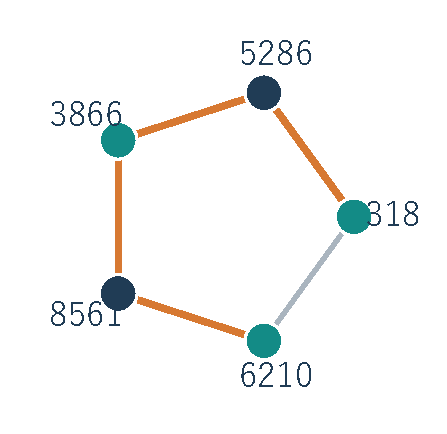
\includegraphics[width=\linewidth]{g70_odd_cycle.pdf}
\end{minipage}\hfill
\begin{minipage}{.57\textwidth}
\textbf{G70にも、実際に5頂点の輪がある。}\\[2mm]
318 → 5286 → 3866 → 8561 → 6210 → 318。入力に5辺とも存在することを確認した。G70には三角形がなくても、全辺を同時にcutできるわけではない。
\end{minipage}
\figcap{11}{G70で確認した閉路。数字は入力の頂点番号。位置と割当ては説明用で、CIM出力を描いたものではない。}

\sub{奇数の輪を数えるだけでは、失点は決まらない}
二つの奇数閉路が同じ辺を共有すると、その1辺を未cutにすることで両方の矛盾を解消できることがある。したがって「奇数閉路が10個あるから10点失う」とは数えられない。\textbf{閉路どうしの重なり方と、実際の未cut辺}を対応させて見る。

\noindent\textcolor{teal}{ここまでは、辺と符号の組合せを見た。次は、CIMの連続的な振幅がどんな形に増えやすいかを見る。}
\source{図10は説明用。図11は実入力の確認結果[7]。}

\newpage
\pagehead{09 / CIMの振幅へ話を進める}{固有ベクトルは「同じ倍率で変わる配置」}{CIMでは結合を通じて振幅が変わる。その変化の方向を読む準備。}
隣の値を足す操作を考える。グラフの辺がある場所を1、ない場所を0とした表が\textbf{隣接行列$A$}である。頂点上の値を並べた$x$に$A$を掛けると、各頂点に隣の値の合計が入る。

\begin{center}
\begin{tikzpicture}
\foreach \n/\xx/\yy/\val/\col in {a/0/1.8/1/teal,b/1.8/1.8/-1/navy,c/1.8/0/1/teal,d/0/0/-1/navy}{\node[circle,fill=\col,text=white,minimum size=10mm,font=\bfseries] (\n)at(\xx,\yy){\val};}
\foreach \aa/\bb in {a/b,b/c,c/d,d/a}{\draw[light,thick](\aa)--(\bb);}
\node[box,text width=76mm] (ex) at (7.5,.9) {左上の値は $+1$\\隣の二つは $-1$ と $-1$\\合計は $-2$：元の値の $-2$ 倍};
\draw[flow](a.east)--(ex.west);
\end{tikzpicture}
\end{center}
\figcap{12}{四角形に交互の数値を置く例。緑・紺は正負、灰は接続。どの点でも、隣を足した結果は元の値の$-2$倍になる。}
\[
A=\begin{pmatrix}0&1&0&1\\1&0&1&0\\0&1&0&1\\1&0&1&0\end{pmatrix},\quad
x=\begin{pmatrix}1\\-1\\1\\-1\end{pmatrix},\quad
Ax=\begin{pmatrix}-2\\2\\-2\\2\end{pmatrix}=-2x.
\]
行列では左上から時計回りに頂点を並べた。各点がばらばらに変わるのでなく、配置全体が同じ倍率で変わっている。このとき、配置$x$が\textbf{固有ベクトル}、倍率$-2$が\textbf{固有値}である。

\sub{Max-Cutとの接点は、隣と逆符号になる方向}
正重みの辺をcutするには、隣と異なる符号が望ましい。隣接行列$A$の負側の固有値に対応する配置は、そのような関係を読む手掛かりになる。[3] ただし一般には値の大きさも点ごとに違い、符号だけを取れば必ず最適解になるわけではない。

\begin{point}{CIMでは、何に使うのか}
結合によって増えやすい振幅の配置と、CIMが実際に作った配置を比べたい。固有値はそのための道具の一つである。\textbf{どの行列を使った固有値か}を、次ページで区別する。
\end{point}
\source{スペクトルとMax-Cutの接点は[3]。4点の計算は本資料の説明例。}

\newpage
\pagehead{10 / 行列の役割を分ける}{つながり方と、CIMの増幅は別の問い}{「固有値が大きい・小さい」の前に、何を測るかを決める。}
\sub{問いA：二つの塊は、どれほどつながっているか}
\pic{spectral_connectivity.pdf}{43mm}
\figcap{13}{同じ二つの四角形を、重み0、0.2、1の辺でつなぐ説明例。緑は頂点、灰は重み1の辺、橙は接続辺。値は正規化ラプラシアンの第2小固有値。G-setでの測定値ではない。}
この例では接続が強いほど値が増える。正規化ラプラシアンは$L=I-D^{-1/2}AD^{-1/2}$で、$D$は各点につながる重みの合計を対角に並べた行列である。辺を持つ連結グラフでは、第2小固有値は正になる。

G55・G70には離れた成分がある。その全体で0が出ても、中心部分のつながり方を比較したことにはならない。\textbf{比較対象を中心部分などにそろえてから使う}。

\sub{問いB：CIMでは、どの振幅の配置が増えるか}
本リポジトリのMax-Cut結合は$J=-\alpha A$（$\alpha>0$）。正の隣接行列$A$とは符号が逆である。[7]
\begin{center}
\begin{tikzpicture}
\node[box,text width=39mm] (a) at (0,0) {\textbf{初期の振幅}\\様々な配置が混ざる};
\node[box,text width=39mm] (b) at (5.3,0) {\textbf{結合による変化}\\方向ごとに倍率が違う};
\node[box,text width=39mm] (c) at (10.6,0) {\textbf{出力の偏り}\\一部の配置が強くなる};
\draw[flow](a)--(b);\draw[flow](b)--(c);
\end{tikzpicture}
\end{center}
\figcap{14}{増幅の考え方を示す説明図。全てのCIM出力がこの一つの要因だけで決まる、という意味ではない。}
初期の小振幅を線形近似し、一回の更新を$c_{t+1}\simeq g_t(aI+bJ)c_t+\text{雑音}$と書く。$c_t$は全頂点の振幅、$a$は自分の振幅を残す係数、$b$は結合の係数、$g_t$は共通の増幅を表す。$Jv=\mu v$の方向は、同じ近似で$g_t(a+b\mu)$倍される。これが固有方向を調べる理由である。

\begin{caution}{どこまで分かっていて、どこからが仮説か}
既存解析ではG55・G70の特定の固有方向への偏りが観測された。[7] ただし実際のCIMには飽和・雑音・時間変化がある。固有値だけでG22との成績差を説明し切ったわけではない。
\end{caution}
\source{[7]。線形近似は増幅の説明用で、実装の完全な更新式ではない。}

\newpage
\pagehead{11 / 最初に読む先行研究}{MQLib：構造から、合う探索法を選ぶ}{ここまで見た構造量が、探索法との相性を読む助けになるかを考える。}
\sub{何をした研究か}
Dunning・Gupta・Silberholzは、Max-Cut/QUBOの37探索法を比較し、58種類の問題特徴から、どの探索法が良い結果を出しそうかを予測した。[1] それぞれの手法に対して、5回の試行平均が比較対象中で最良になるかを学ぶランダムフォレストを作る。

\begin{center}
\begin{tikzpicture}
\node[box,text width=39mm] (a) at (0,0) {グラフ1個\\58種類の特徴量};
\node[box,text width=39mm] (b) at (5.3,0) {各探索法の\\有望さを予測};
\node[box,text width=39mm] (c) at (10.6,0) {1手法を選び\\その問題を解く};
\draw[flow](a)--(b);\draw[flow](b)--(c);
\end{tikzpicture}
\end{center}
\figcap{15}{論文の処理を整理した図。選ぶ対象は探索法。同じグラフ上の個々のCIM候補を選ぶ実験ではない。}

\sub{何が分かったか}
2,635問題を学習1,844・評価791に分けた実験で、1手法を選ぶ構成の平均期待偏差は0.08\%。比較に使われたBUR02という1手法を全問題で固定使用した場合は0.27\%だった。[1, Section 6]
\pic{mqlib_result.pdf}{43mm}
\figcap{16}{論文の報告値を再描画。小さいほど論文内の最良既知値に近い。灰はBUR02固定、緑は問題ごとに探索法を選んだ場合。本研究での再実験ではない。}

\begin{point}{この研究から借りたい考え方}
「普遍的な難しさ」を1個の数字にする前に、\textbf{ある構造で、ある探索法がどう振る舞うか}を見る。今回なら、グラフ構造とCIM条件を対応させ、どこに未cut辺や配置の偏りが残るかを調べる。
\end{point}
\sub{読む場所と、まだ言えないこと}
\textbf{Section 2.2}で特徴量、\textbf{Section 6}で探索法選択と評価を読む。特徴量で手法の相性を予測できたことは、個々のCIM解の「将来良い種になる価値」まで証明したことではない。
\source{[1]の著者公開本文。偏差の基準は最良既知値であり、全問題の厳密最適値ではない。}

\newpage
\pagehead{12 / 解の状態も見る先行研究}{ECO-DQN：今の配置から、次の一手を選ぶ}{グラフ構造に加え、現在の解の情報をどう使うかを見る。}
ECO-DQNは、\textbf{1頂点を選んで符号を反転する}操作を繰り返す。前に動かした頂点を再び動かせるので、一度の判断をやり直せる。MPNNは辺を通じて情報を集め、各頂点の反転に対するQ値を予測する。[6]

\begin{center}
\begin{tikzpicture}
\node[box,text width=39mm] (a) at (0,0) {グラフ＋現在の配置\\探索の履歴};
\node[box,text width=39mm] (b) at (5.3,0) {MPNNが\\各反転のQ値を予測};
\node[box,text width=39mm] (c) at (10.6,0) {1頂点を反転\\状態を更新};
\draw[flow](a)--(b);\draw[flow](b)--(c);
\draw[flow](c.south)--++(0,-.7)-|(a.south);
\end{tikzpicture}
\end{center}
\figcap{17}{ECO-DQNの1ステップ。動くたびに状態が変わり、評価をやり直す。[6]}

\sub{「すぐ増える得点」と「Q値」は違う}
ある頂点に未cut辺が3本、cut辺が1本つながっていれば、その頂点の反転で3本がcutになり、1本が未cutになる。直後の変化は$3-1=+2$点。この\textbf{即時の改善量（gain）}は、学習せずに計算できる。

一方、Q値は\textbf{その一手の後にも探索を続けたときの報酬}を予測する。ECO-DQNでは過去最高cutを更新した分を頂点数で割って主報酬とし、初めて訪れる局所最良状態への補助報酬も使う。一時的な悪化には直接罰を与えず、先の改善を探れるようにしている。[6]

\begin{point}{モデルは、何を見ているか}
\textbf{頂点ごと：}現在の符号、反転直後のgain、最後の反転からの手数。\\
\textbf{全体：}過去最良cutとの差、過去最良配置との距離、すぐ改善できる反転の数、残り手数。\\[1mm]
この7観測から、構造だけでなく\textbf{今どこまで探索が進んだか}も読む。
\end{point}
\sub{今回の関心に近いのは、どの部分か}
CIM出力についても「どこに改善できる点が残るか」は計算できる。まずはECO-DQNの観測の考え方を借り、\textbf{CIMの解を理解する診断}に使う。GA/SAに渡した後の価値をQ値と同一視はしない。
\source{[6]のObservations・Rewards。3対1の例は本資料の説明例。}

\newpage
\pagehead{13 / ECO-DQNの結果を正しく読む}{参考になる成果と、今回まだ確かめていないこと}{CIMとの関係を、実験済みの事実と応用案に分ける。}
\sub{論文で報告されたこと}
200頂点のERグラフで学習したモデルをG-setに適用したTable 1では、「G22--32」群の平均比率がECO-DQNで0.971、S2V-DQNで0.919だった。[6] 基準cut値に対する得点の比であり、\textbf{G22単独の結果でも、最適解に到達する確率でもない}。この群は各グラフ1エピソードの評価である。

補足資料には\textbf{SimCIMとの比較}もある。ただし、CIMが作った解をECO-DQNに渡す結合実験ではなく、本リポジトリの進行波CIMとSimCIMも同一実装ではない。

\begin{center}
\begin{tikzpicture}
\node[box,text width=39mm] (a) at (0,0) {\textbf{CIM}\\解と時間軌跡を出す};
\node[box,text width=39mm] (b) at (5.3,0) {\textbf{観測量を計算}\\gain・失点・配置};
\node[box,text width=39mm] (c) at (10.6,0) {\textbf{構造と照合}\\どこで偏るかを読む};
\draw[flow](a)--(b);\draw[flow](b)--(c);
\end{tikzpicture}
\end{center}
\figcap{18}{今回の資料からの利用案。CIMを解生成の中心に置き、観測量で出力を診断する。ここにECO-DQN学習器を実装済みという意味はない。}

\sub{そのまま導入する前に残る、三つの課題}
\begin{enumerate}
\item \textbf{Q値の意味が違う。} ECO-DQN自身の報酬と行動方針に対する予測であり、GA/SAの初期解としての将来価値ではない。
\item \textbf{CIM出力には探索履歴がない。} 「最後の反転から何手」などの観測は、そのままでは決まらず、初期化を設計する必要がある。
\item \textbf{対象と計算費用が違う。} 学習時のグラフ分布からG55・G70へ移す性能や、10,000頂点で毎手推論する負荷は、この資料では未検証である。
\end{enumerate}

\begin{point}{現段階で取り入れる範囲}
まずは学習器を追加せず、反転gainや未cut辺の位置をCIM出力から計算する。その結果で不足する情報が分かってから、学習モデルが必要かを判断する。
\end{point}
\source{報告値・SimCIM比較は[6]。CIM診断への利用は本資料の提案。}

\newpage
\pagehead{14 / 話を研究目的へ戻す}{次に知りたいのは、CIMが「どこで失点するか」}{構造の説明を、測れる問いへつなぐ。}
ここまでで、G55・G70を木と中心部分に分ける意味、次数とcoreの違い、中心部分の閉路、振幅の固有方向を整理した。これらを使い、まず三つの問いを立てる。

\begin{point}{問い1：失点は、木と中心部分のどちらにあるか}
各CIM解の未cut辺を分けて数える。橋側の未cutは、部分全反転で改善できる余地を示す。中心部分の未cutは、閉路の制約と実際の探索状態を調べる対象になる。
\end{point}
\begin{point}{問い2：異なる解が、同じ場所で失敗していないか}
全頂点の符号を単純に比較するだけでなく、どの辺がcut・未cutになったかを比べる。孤立点の符号や全体反転による違いを除いて、中心部分の共通した配置を見る。
\end{point}
\begin{point}{問い3：配置の偏りは、振幅の増幅と対応するか}
CIMの結合行列$J$の固有方向と、保存された振幅や符号配置を照合する。特定の方向へ寄ることが、得点や未cut辺の位置とどう関係するかを調べる。
\end{point}

\sub{Transformerは、何を足せそうかが見えてから}
GraphGPS [4]は局所の情報交換と全体のattentionを組み合わせる。MARCO [5]はGraph Transformerを組合せ最適化の探索に使う。ただし、モデル名を先に決めるより、\textbf{次数・gain・閉路などの観測だけでは表せない情報が何か}を先に明らかにしたい。

\sub{将来の候補評価へ戻る条件}
構造とCIM出力の関係が整理できた後で、「その情報がGA/SAへ渡す初期解の良さを予測するか」を検証する。同じグラフでは構造量だけで候補の差は付かないため、\textbf{候補ごとの配置情報}との組合せが必要になる。価値関数や学習データの詳細設計は、その段階の課題として残す。

\begin{caution}{この資料の結論の範囲}
G22の成績が良い原因や、CIM解の将来価値を予測する評価関数が完成したわけではない。今回できたのは、\textbf{どの構造の、どの振る舞いを観測すれば説明を進められるか}を具体化したことである。
\end{caution}

\newpage
\pagehead{15 / 参照先と再現情報}{本文で使った根拠を、たどれるようにする}{報告値・入力の集計・説明用の例を区別する。}
{\small
\noindent\textbf{[1] Dunning, I.; Gupta, S.; Silberholz, J. (2018).}\\
\textit{What Works Best When? A Systematic Evaluation of Heuristics for Max-Cut and QUBO.} INFORMS Journal on Computing, 30(3), 608--624.\\
\href{https://raw.githubusercontent.com/MQLib/MQLib/master/paper/SECM_final.pdf}{著者公開本文} / \href{https://github.com/MQLib/MQLib}{公式実装}。Section 2.2・6。図16は報告値の再描画。

\noindent\textbf{[2] Rehfeldt, D.; Koch, T.; Shinano, Y. (2023).}\\
\textit{Faster exact solution of sparse MaxCut and QUBO problems.} Mathematical Programming Computation, 15, 445--470.\\
\href{https://doi.org/10.1007/s12532-023-00236-6}{公開本文・DOI}。Section 4.1の分解を参照。橋の数値例は本資料で作成。

\noindent\textbf{[3] Trevisan, L. (2009; preprint 2008).}\\
\textit{Max Cut and the Smallest Eigenvalue.} STOC 2009.\\
\href{https://arxiv.org/abs/0806.1978}{arXiv:0806.1978}。非負重みMax-Cutとスペクトルの接点。

\noindent\textbf{[4] Rampášek, L. et al. (2022).}\\
\textit{Recipe for a General, Powerful, Scalable Graph Transformer.} NeurIPS 2022.\\
\href{https://arxiv.org/abs/2205.12454}{arXiv:2205.12454}。GraphGPS。効率的attentionを選べる構成。

\noindent\textbf{[5] Garmendia, A. I. et al. (2024).}\\
\textit{MARCO: A Memory-Augmented Reinforcement Framework for Combinatorial Optimization.} IJCAI 2024, 6931--6939.\\
\href{https://www.ijcai.org/proceedings/2024/0766.pdf}{公開本文}。Section 5のGraph Transformer。

\noindent\textbf{[6] Barrett, T. D.; Clements, W. R.; Foerster, J. N.; Lvovsky, A. I. (2020).}\\
\textit{Exploratory Combinatorial Optimization with Reinforcement Learning.} AAAI, 34(04), 3243--3250.\\
\href{https://ojs.aaai.org/index.php/AAAI/article/view/5723}{出版版} / \href{https://arxiv.org/abs/1909.04063}{本文・補足資料} / \href{https://github.com/tomdbar/eco-dqn}{公式実装}。観測・報酬・Table 1・SimCIM比較。

\noindent\textbf{[7] 本リポジトリの入力・記録・実装。}\\
\texttt{input/G22.txt, G55.txt, G70.txt}、\texttt{modules/CIM.py}、8月23日のCIM解析、9月14日のGA世代別多様性測定。本文の性能値は既存結果で、新規実験ではない。

\noindent\textbf{[8] NetworkX：k-coreの定義と実装。}\\
\href{https://networkx.org/documentation/stable/reference/algorithms/generated/networkx.algorithms.core.k_core.html}{公式ドキュメント}。本資料の集計環境はNetworkX 3.6.1。
}
\sub{今回の追加集計と、図の再現}
{\small
図5の内訳は\texttt{data/decomposition.json}に保存した。図9の次数、図11のG70閉路、図13の説明用固有値も同梱データから再現できる。説明用の小グラフと、実入力の集計値は各図の説明に明記した。

\texttt{make\_second\_revision\_figures.py}で追加集計と図を再生成できる。旧版から継続する図のコード、TeX、データはソースZIPに同梱。赤字ごとの反映先は\texttt{redline\_response.md}に記録した。
}
\end{document}
